\documentclass[../main/main.tex]{subfiles}

\newdate{date}{02}{10}{2020}



\begin{document}



\chapter{Basics Definitions and Compartmental Models}

\begin{chapquote}{Unknown author}
Some models are wrong, but most of them are useful.
\end{chapquote}


\marginpar{ \textbf{Lecture 2.} \\  \displaydate{date}. \\ Compiled:  \today.}

Models in science have two different roles: \textbf{understanding} what happens and \textbf{prediction}.
There are two types of models: one more simple and one more complex. In the simplest one you just consider the minimal number of parameters and events involved: this allow to understand what are the main mechanism of a phenomena.

In this course, we gonna start with very simple models in which we firstly assume that there are no structures in the population. This is not accurate, but allows us to understand at a first glance some underlying mechanism.
Then, we will consider social structures and contact network models. We will also take into account the interaction of different populations and we analyze how data move from one population to the other. At last, there is another class of models called “Agent Based” models, but we will only brief introduct it.

\section{Comportamental models}

We introduce the \textbf{comportamental models} in which most based epidemiologist theories are based on. In reality, there are different levels of understanding how the diseases diffuse, as for instance at a biological level or a more simplest one. It is impossible to insert all the details of a process in a models. We need to summarize all the biological process in few parameters which are the average of what you see inside the population. This is the same principle behind the statistical mechanics in which we concentrate for large scale effects.

\begin{figure}[!b]
\centering
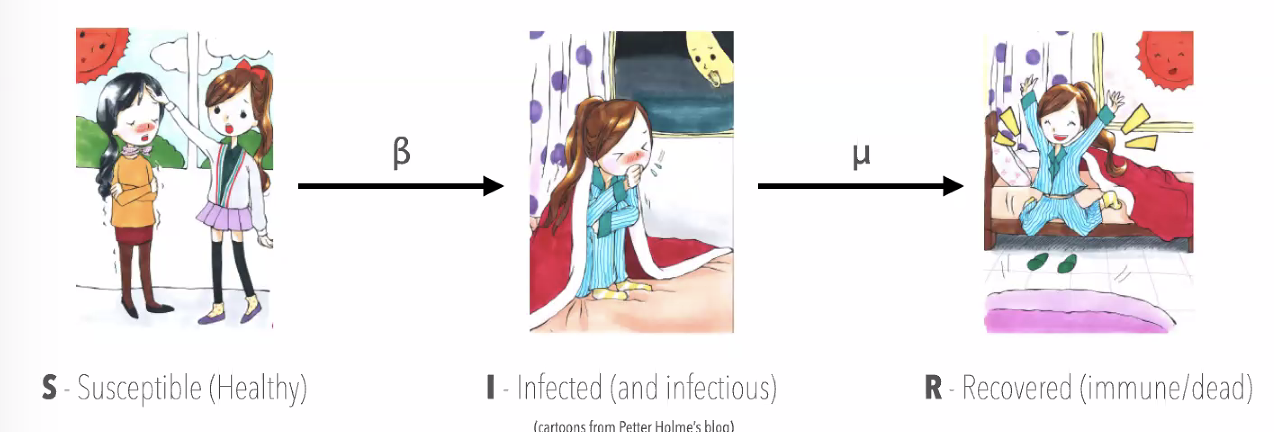
\includegraphics[width=0.9\textwidth]{../lessons/image/02/1_classification.png}
\caption{\label{fig:1_classification} Classification of infected population in three different stage of the disease.}
\end{figure}

Let us consider a population of any individuals and try to characterize them. For instance we have three compartments and we want to classify people according to the state of their diseases, as in Fig. \ref{fig:1_classification}. We have also transition from one state to the other with rates as \( \beta  \) and \( \mu  \) which describes the dynamic of the diseases
The only problems it is that this approximation is quite strong, because by fixing the rates we are assuming that the process underlying is a Markovian one. In reality, you do not have a exponential distribution but a decay. This will be seen in the course when we will talk about “non-Markovian” epidemics. For instance the \( \beta  \) can be the “per contact” infectous rate, so you are just counting the number of contacts.
As examples we can consider different models which depend on the type of disease as SI, SIS, SIR and so on and so forth.

There are difference between medical status and infection status. We do not care about medical status but only about the disease and how the immuning system is reacting.
We have four main stages of the disease: starting from a helthy state, the individual can contract the disease and then it become infectious until it recover (Fig. \ref{fig:2_5}). The most important things is that the compartments are not the same of the medical status.

\begin{figure}[h!]
\centering
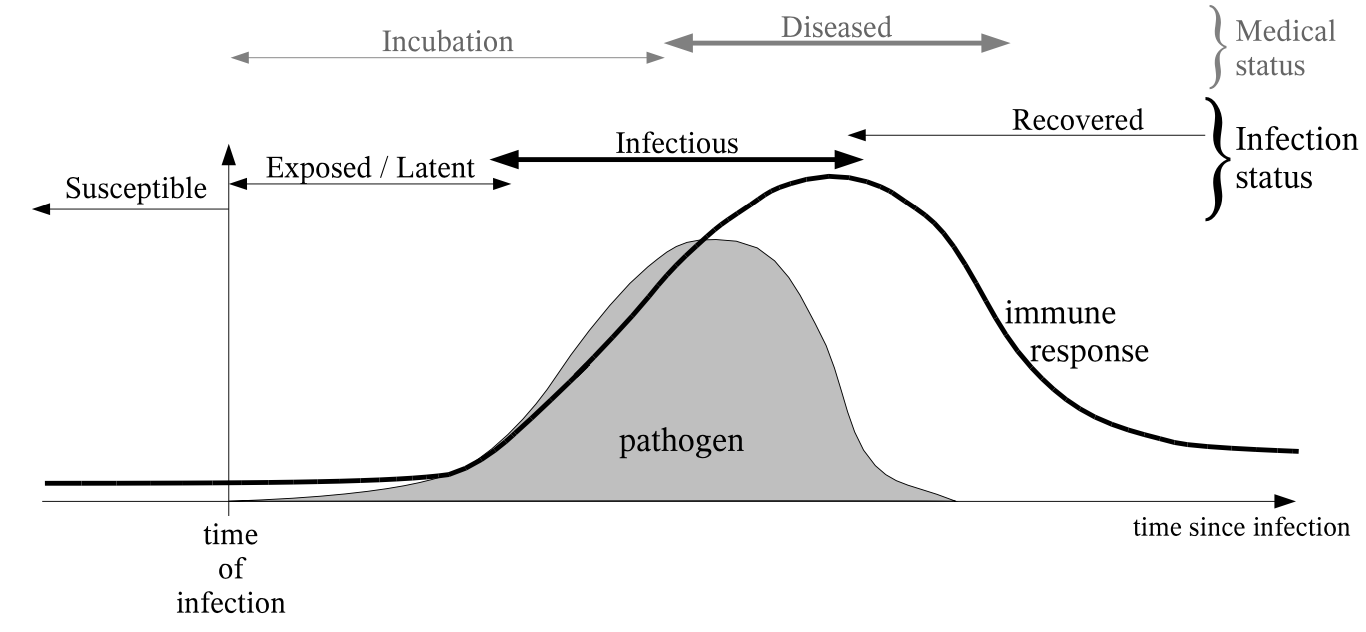
\includegraphics[width=0.7\textwidth]{../lessons/image/02/5.png}
\caption{\label{fig:2_5} A caracature of the time-line of infection, showing the dynamics of the pathogen (gray area) and the host immune response (black line) as well as labeling the various infection classes: susceptible, exposed, infectious, and recovered. Note that the diseased period, when symptoms are experienced, is not necessarily correlated with any particular infection class.}
\end{figure}

Now, let us introduce the \textbf{Basic Reproductive Number} \( R_0 \) (pronunced \( R \) naught) which is a measure of the infection of the population. We put one guy inside a group for instance for three days and at the end of these days we count the number of secondary cases that we have. This is the main idea of \( R_0 \). This number determines wheter a disease will spread or not:
  \begin{equation}
    \begin{cases}
     R_0 < 1\\
     R_0 = 1\\
     R_0 > 1\\
    \end{cases}
  \end{equation}
Let us consider the plot of Fig. \ref{fig:2_R_0.png}, we have a sort of second order phase transition at the point \( R_0=1 \).
Note that the \( R_0 \) number for the SARS is higher thant the one of COVID-19, but we did not experienced an outbreak of this disease.
For computing \( R_0 \) we are assuming that the population is totally susceptible, but this assumption is valid only at the very early stages. Then, we care ombining also epidemiological and demographical features. The conclusion is that this number could vary from one population to another.
Since we are doing a coarse-graining of the dynamics, the number \( R_0 \) represents the mean of possibly different distributions. It can give the wrong idea of similar \( R_0 \), means similar outbreaks.
The distribution of infections can be quite heterogeneous, hence the mean could be quite representive in homogeneous populations. For instance, let us consider the plot in Fig. \ref{fig:3_outbreaks}. We see that SARS is etherogeneous, while Spanish Flu was a homogeneous one.
The COVID-19 is most likely somewhere in the middle.

\begin{figure}[h!]
\centering
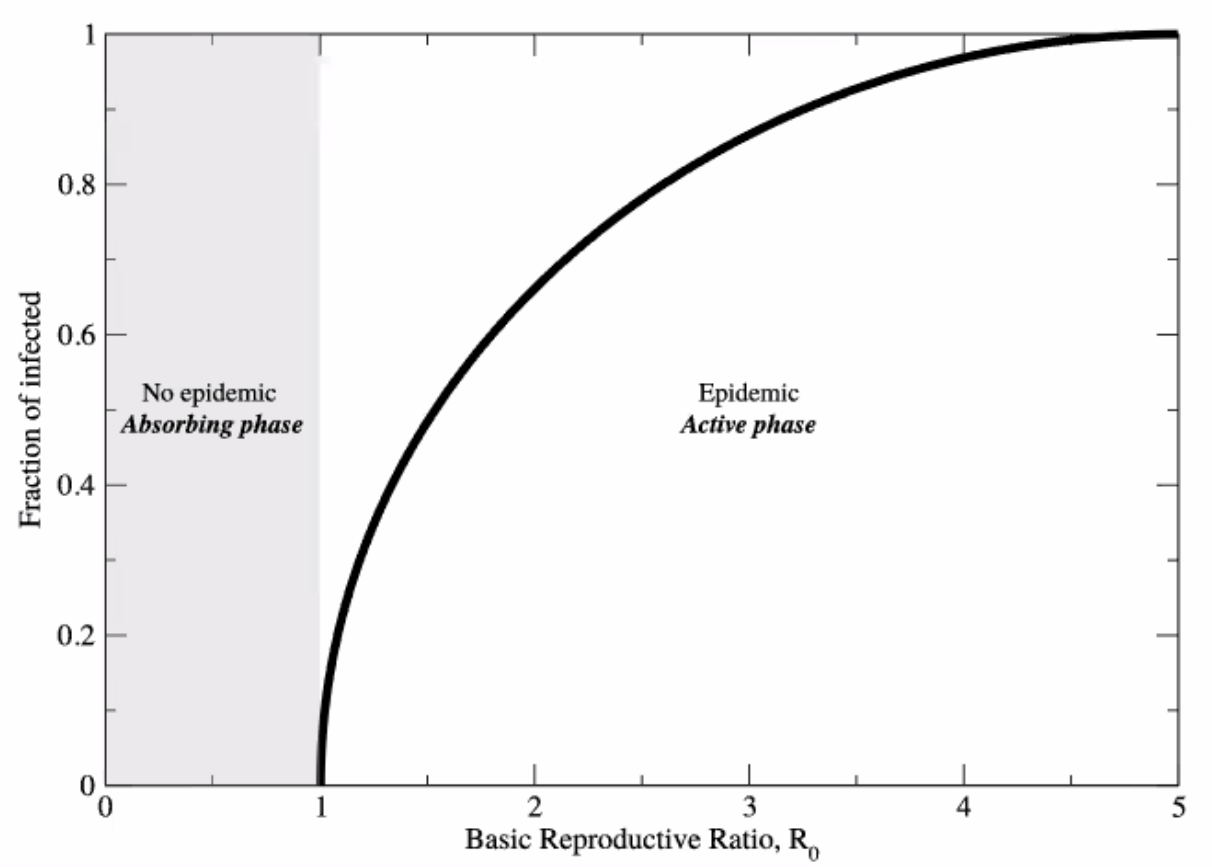
\includegraphics[width=0.7\textwidth]{../lessons/image/02/2_R_0.png}
\caption{\label{fig:2_R_0.png} Fraction of infected vs basic Reproductive Ratio, \( R_0 \).}
\end{figure}

\begin{figure}[h!]
\centering
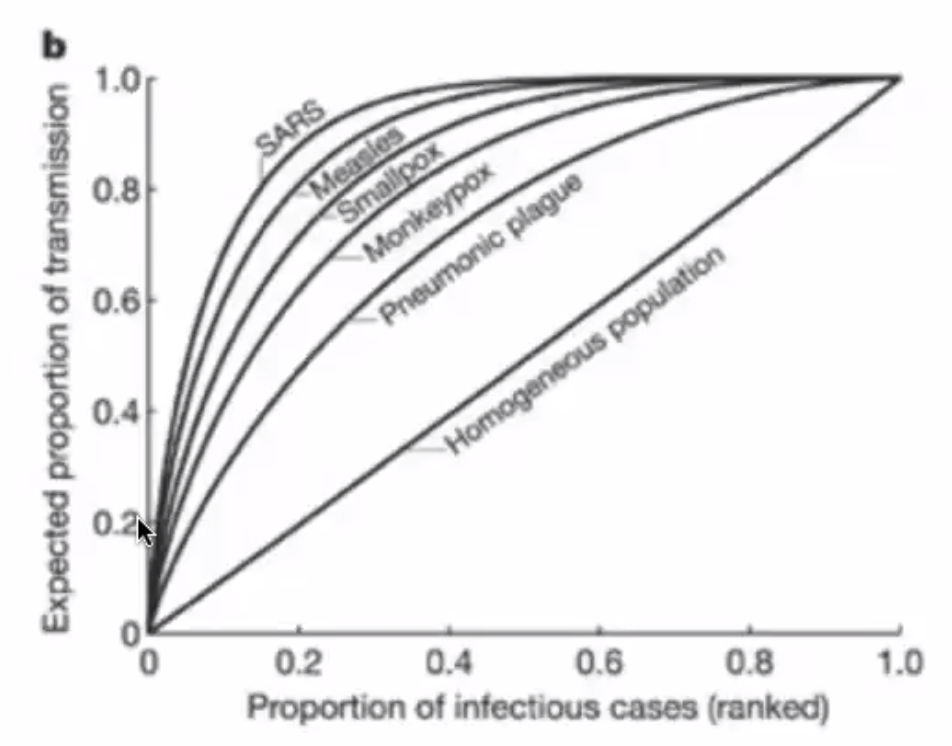
\includegraphics[width=0.6\textwidth]{../lessons/image/02/3_outbreaks.png}
\caption{\label{fig:3_outbreaks} Figure from: Lloyd-Smith et al. Nature 438, 355–359 (2005).}
\end{figure}

\begin{figure}[h!]
\centering
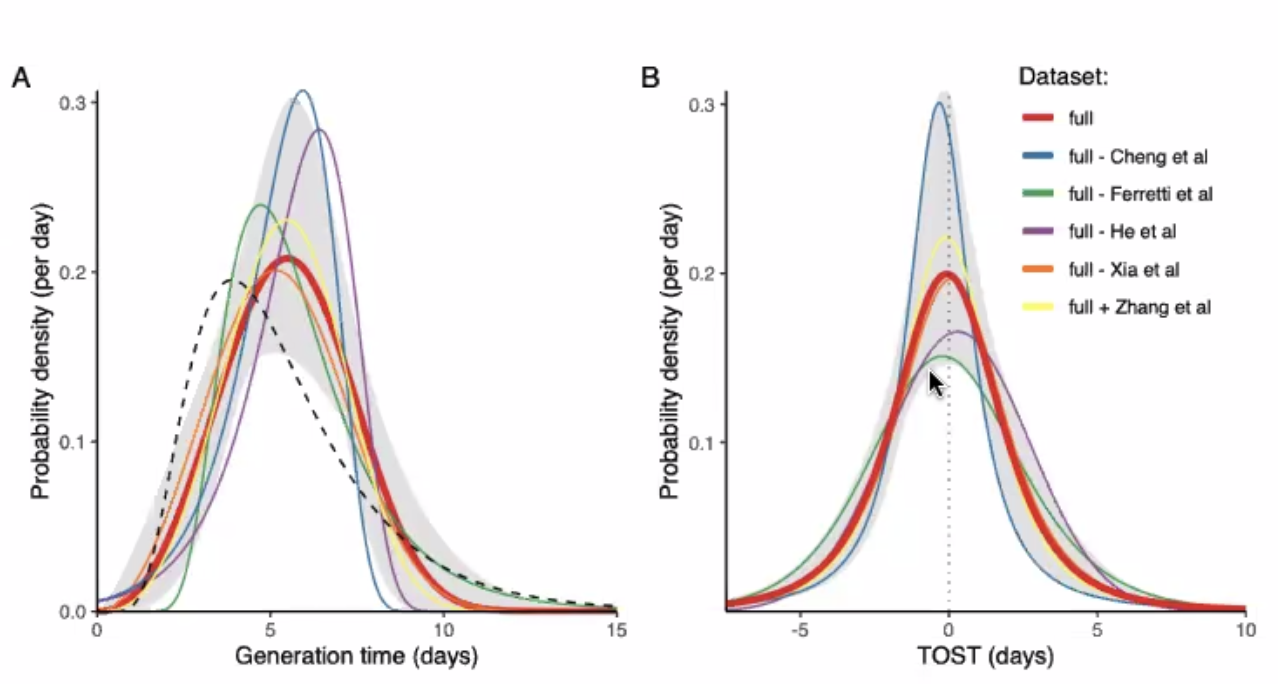
\includegraphics[width=0.6\textwidth]{../lessons/image/02/4_TOST.png}
\caption{\label{fig:4_TOST} Figure from: Ferretti et al. \url{https://www.medrxiv.org/content/10.1101/2020.09.04.20188516v1}}
\end{figure}

Now, we introduce the \textbf{Effective Reproductive Number} \( R(t) \), which is the same of \( R_0 \) but it varies in time. Hence, it is the average number of secondary cases a case produces in a population at time \( t \).
Another important quantity is the \textbf{Infectious period}:
\begin{equation}
  \tau = \frac{1}{\mu }, \quad \tau = \frac{1}{(\alpha + \mu )}
\end{equation}
Other relevant quantities are the \textbf{Incubation period} (from infection to symptoms), the \textbf{Generation time} (from infection to infection), the \textbf{Serial interval} (from symptoms to symptoms) or the \textbf{TOST} (measures from symptoms to infection). The problems is that TOST in many cases can be negative (see Fig. \ref{fig:4_TOST} for more details).










\end{document}
